\section{Lecture 3. Efficient Pattern Mining Methods}
\subsection{The Downward Closure Property of Frequent Patterns}
The downward closure (also called <<Apriori>>) property of frequent patterns: \textbf{Any subset of a frequent itemset must be frequent}. Apriori pruning principle: \textbf{If there is any itemset which is infrequent, its superset should not even be generated!}\\

Scalable mining Methods: Three major approaches
\begin{itemize}
\item Level-wise, join-based approach: Apriori (\ref{apriori})
\item Vertical data format approach: Eclat (\ref{eclat})
\item Frequent pattern projection and growth: FPgrowth (\ref{fpgrowth})
\end{itemize}

%--
\subsection{The Apriori Algorithm}\label{apriori}
\subsubsection{Algorithm pseudocode}
$C_k$: Candidate itemset of size k

$F_k$ : Frequent itemset of size k

TDB = transactional database\\

\begin{algorithm}
\caption{The Apriori Algorithm}
\begin{algorithmic}
\State $k := 1$
\State $F_k :=$ frequent items \Comment{frequent 1-itemset}
\While{$F_k \neq \varnothing$}
    \State $C_{k+1} :=$ candidates generated from $F_k$ \Comment{candidate generation}
    \State Derives $F_{k+1}$ by counting candidates in $C_{k+1}$ with respect to TDB at minsup
    \State $k := k + 1$
\EndWhile
\State \Return $\cup_k F_k$  \Comment{return F\textsubscript{k} generated at each level}
\end{algorithmic}
\end{algorithm}

%--
\subsubsection{How to generate candidates?}

\begin{itemize}
\item Step1: self-joining F\textsubscript{k}
\item Step2: pruning
\end{itemize}


\begin{algorithm}
\caption{Step1: self-joining F\textsubscript{k}}
\begin{algorithmic}
\State insert into C\textsubscript{k}
\State select p.item\textsubscript{1}, p.item\textsubscript{2}, ..., p.item\textsubscript{k-1}, q.item\textsubscript{k-1}
\State from F\textsubscript{k-1} as p, F\textsubscript{k-1} as q
\State where p.item\textsubscript{1}= q.item\textsubscript{1}, ..., p.item\textsubscript{k-2} = q.item\textsubscript{k-2}, p.item\textsubscript{k-1} < q.item\textsubscript{k-1}
\end{algorithmic}
\end{algorithm}

\begin{algorithm}
\caption{Step2: pruning}
\begin{algorithmic}
\ForAll{itemsets c in C\textsubscript{k}}
    \ForAll{(k-1) subsets s of c}
        \If{s is not in F\textsubscript{k-1}}
            \State delete c from C\textsubscript{k}
        \EndIf
    \EndFor
\EndFor
\end{algorithmic}
\end{algorithm}    

%--    
\subsection{Extensions or Improvements of Apriori}
\begin{itemize}
\item Reduce passes of transaction database scans 
    \begin{itemize}
    \item Partitioning
    \item Dynamic itemset counting
    \end{itemize}
\item Shrink the number of candidates
    \begin{itemize}
    \item Hashing
    \item Pruning by support lower bounding
    \item Sampling
    \end{itemize}
\item Exploring special data structures
    \begin{itemize}
    \item Tree projection
    \item H-miner
    \item Hypecube decomposition
    \end{itemize}
\end{itemize}  

%--
\subsubsection{Partitioning}
Theorem: \textit{Any itemset that is potentially frequent in TDB must be frequent in at least one of the partitions of TDB}\\

Method: Scan Database Only Twice:
\begin{itemize}
\item Scan 1: Partition database (how?) and find local frequent patterns
\item Scan 2: Consolidate global frequent patterns (how to?)
\end{itemize}

%--
\subsubsection{Direct Hashing and Pruning (DHP)}
Observation: \textit{A k-itemset whose corresponding hashing bucket count is below the threshold cannot be frequent}

%-- 
\subsection{Vertical Data Format}\label{eclat}
\textbf{ECLAT} - Equivalence Class Transformation

Frequent patterns are derived based on vertical intersections. To accelerate data mining you can use \textbf{diffset}: only keep track of differences of tids.

%--
\subsection{A Pattern Growth Approach}\label{fpgrowth}
\textbf{FP-tree} - frequent pattern tree

\begin{figure}[H]
    \centering
    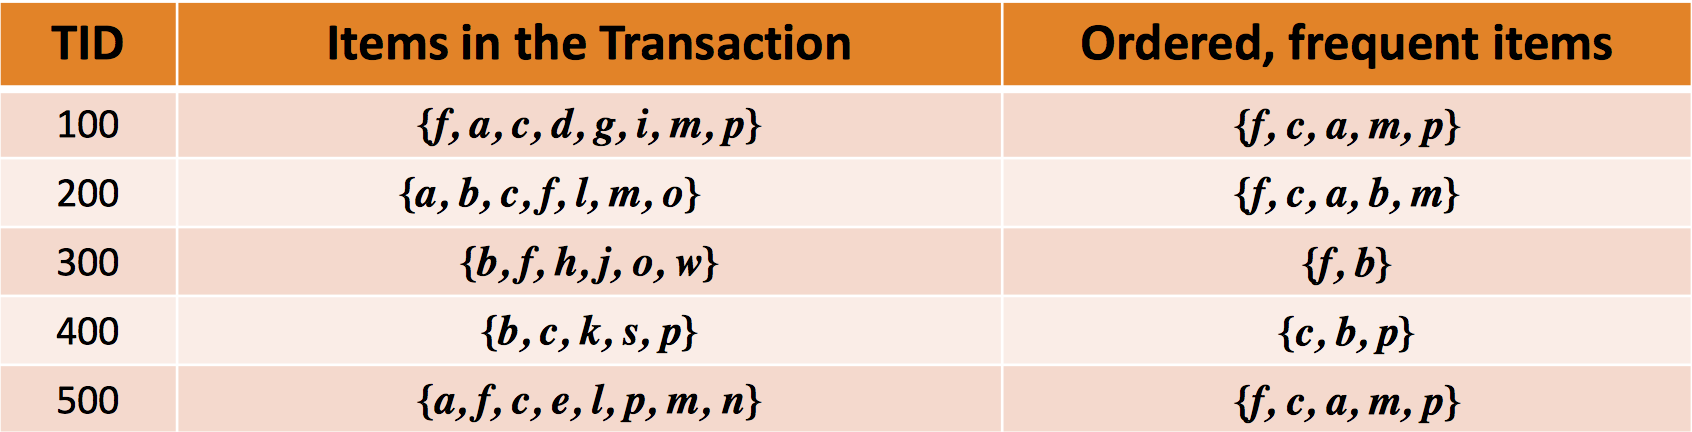
\includegraphics[width=\linewidth]{transactional_db.png}
    \caption{Transational DB}
\end{figure}

\begin{figure}[H]
    \centering
    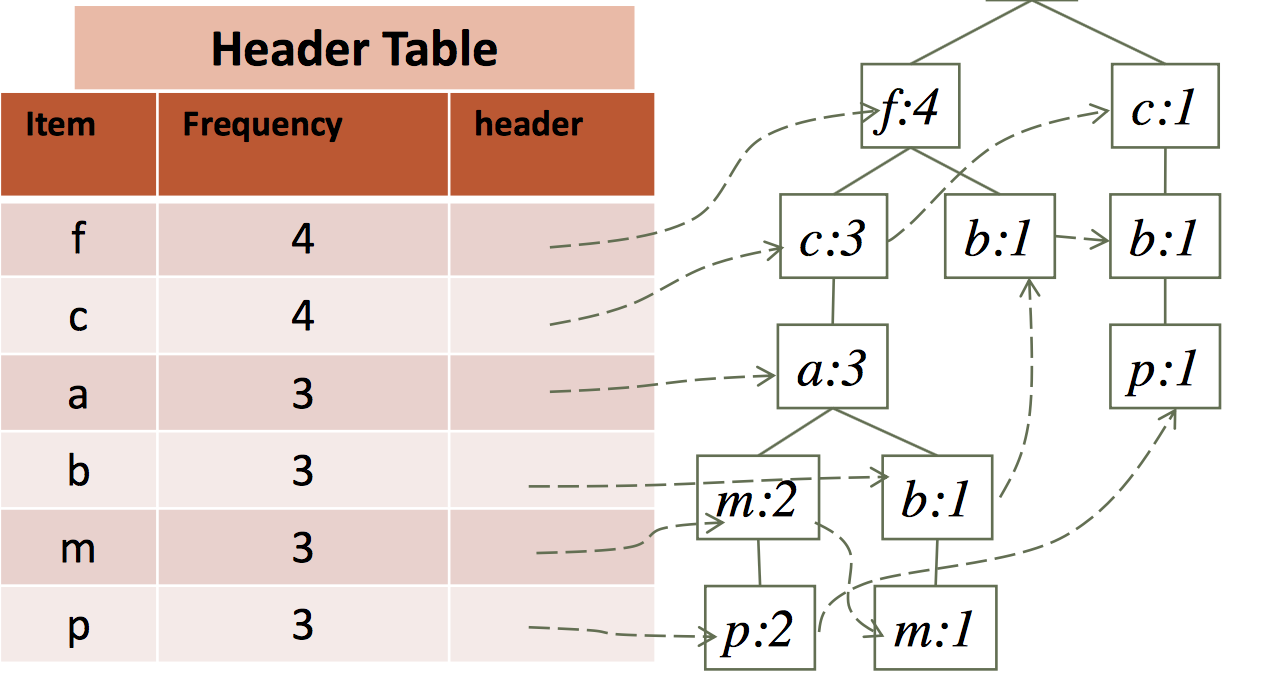
\includegraphics[width=\linewidth]{fptree.png}
    \caption{FP-tree}
\end{figure}

%--
\subsection{CLOSET+: Mining Closed Itemsets by Pattern-Growth}
Itemset merging: \textit{If Y appears in every occurrence of X, then Y
is merged with X}

%--
\subsection{Recommended readings}
\begin{itemize}
\item R. Agrawal and R. Srikant, <<Fast algorithms for mining association rules>>, VLDB'94
\item A. Savasere, E. Omiecinski, and S. Navathe, <<An efficient algorithm for mining association rules in large
databases>>, VLDB'95
\item J. S. Park, M. S. Chen, and P. S. Yu, <<An effective hash-based algorithm for mining association rules>>, SIGMOD'95
\item S. Sarawagi, S. Thomas, and R. Agrawal, <<Integrating association rule mining with relational database systems: Alternatives and implications>>, SIGMOD'98
\item M. J. Zaki, S. Parthasarathy, M. Ogihara, and W. Li, <<Parallel algorithm for discovery of association rules>>, Data Mining and Knowledge Discovery, 1997
\item J. Han, J. Pei, and Y. Yin, <<Mining frequent patterns without candidate generation>>, SIGMOD’00
\item M. J. ZakiandHsiao, <<CHARM: An Efficient Algorithm for Closed Itemset Mining>>, SDM'02
\item J. Wang, J. Han, and J. Pei, <<CLOSET+: Searching for the Best Strategies for Mining Frequent Closed Itemsets>>, KDD'03
\item C. C. Aggarwal, M.A., Bhuiyan, M. A. Hasan, <<Frequent Pattern Mining Algorithms: A Survey>>, in Aggarwal and Han (eds.): Frequent Pattern Mining, Springer, 2014
\end{itemize}